\section{Vehicle Emissions}
\label{sec:Results_Emissions}

The environmental impact of the control strategies is evaluated by focusing on the average \ac{co2} and \ac{nox} mass per kilometre, as detailed in Table~\vref{tab:Emissions}. The results, visualized in Figures~\vref{fig:Emis_692} through \vref{fig:Emis_3462}, are discussed separately for the HBEFA4 and PHEMlight5 models, as their different sensitivities to transient vehicle dynamics yield distinct outcomes.

\paragraph{Low to Intermediate Demand ($69$--$692~\unit{\veh\per\hour}$).}
In the low-to-intermediate demand range, the \ac{eco-glosa} algorithm's performance under the HBEFA4 model is inconsistent. For example, at a demand of $69~\unit{\veh\per\hour}$, it achieves a notable \ac{co2} reduction of nearly $15\%$ at $40\%$ \ac{mpr}, with emissions falling to $127.88~\unit{\gram\per\kilo\metre}$. However, this gain is immediately reversed at $50\%$ \ac{mpr}, where emissions increase to $165.55~\unit{\gram\per\kilo\metre}$. A similar pattern of fluctuation is observed at $692~\unit{\veh\per\hour}$, as illustrated in Figure~\vref{fig:Emis_692_HBEFA4}.
\mynewline
The performance of the more sensitive PHEMlight5 model is also variable. While the \ac{eco-glosa} controller does achieve significant emission reductions at certain penetration rates, it can perform worse than the Standard case at others. This instability means that the simpler, throughput-oriented \ac{flow-glosa} controller can sometimes yield better environmental outcomes. For instance, at $692~\unit{\veh\per\hour}$ and $20\%$ \ac{mpr}, the baseline \ac{flow-glosa} emits $165.46~\unit{\gram\per\kilo\metre}$ of \ac{co2}. This is $1.86~\unit{\gram\per\kilo\metre}$ less than the \ac{eco-glosa} controller under identical conditions, with a marginal corresponding reduction in \ac{nox} as well.

\begin{figure}[htb]
  \centering
  \begin{subfigure}[b]{0.45\textwidth}
    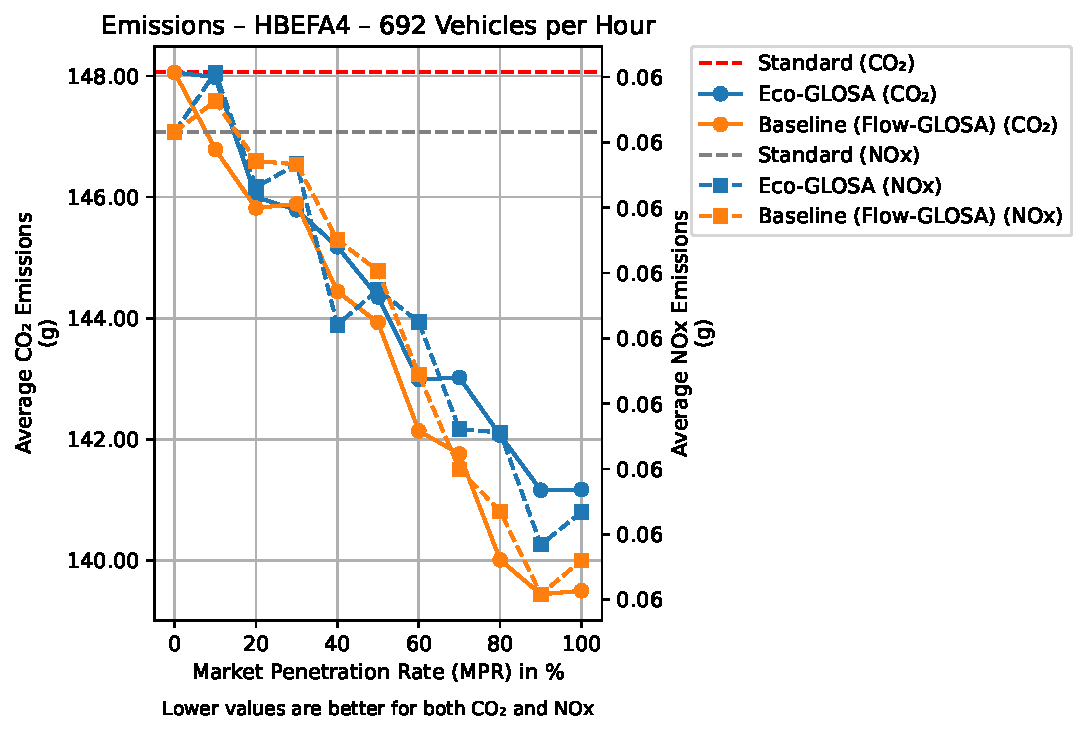
\includegraphics[width=\textwidth]{data/img/Emissions/Emissions_HBEFA4_Cars692.pdf}
    \caption{HBEFA4 at $692\,\mathrm{veh/h}$.}
    \label{fig:Emis_692_HBEFA4}
  \end{subfigure}\hfill
  \begin{subfigure}[b]{0.45\textwidth}
    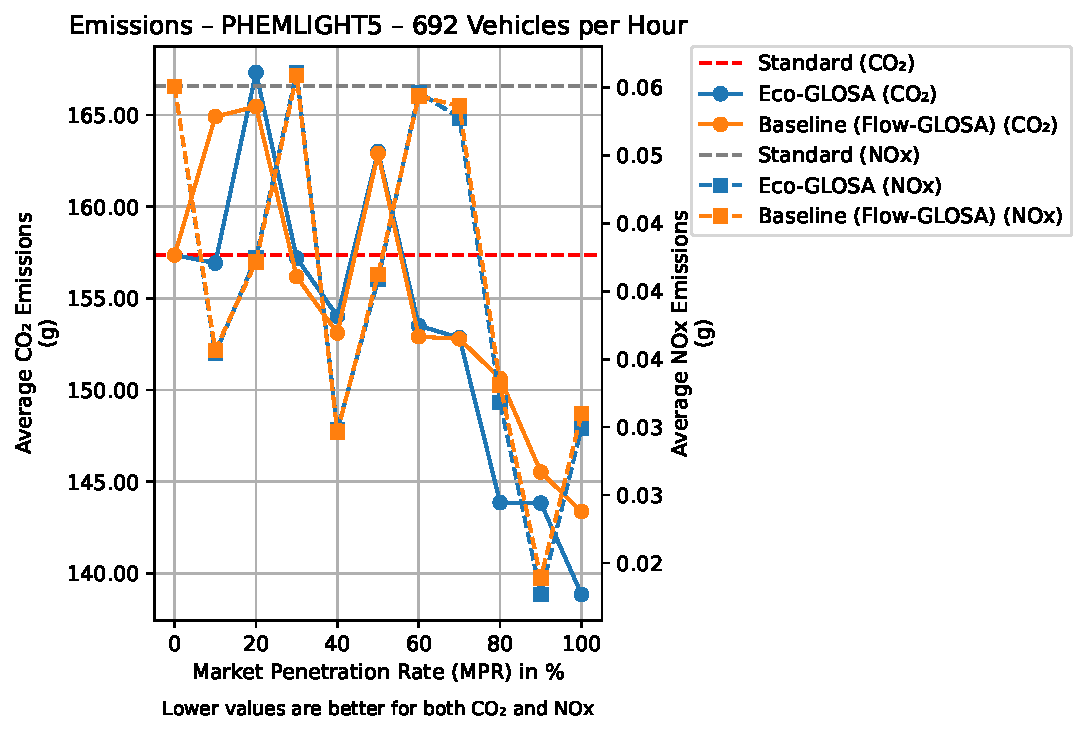
\includegraphics[width=\textwidth]{data/img/Emissions/Emissions_PHEMLIGHT5_Cars692.pdf}
    \caption{PHEMlight5 at $692\,\mathrm{veh/h}$.}
    \label{fig:Emis_692_PHEM}
  \end{subfigure}
  \caption[\ac{co2} and \ac{nox} emissions vs. \ac{mpr} at $692~\unit{\veh\per\hour}$]{\ac{co2} and \ac{nox} emissions versus \ac{mpr} at a low demand of $692~\unit{\veh\per\hour}$.}
\label{fig:Emis_692}
\end{figure}

\paragraph{Emerging Congestion ($1385$--$2077~\unit{\veh\per\hour}$).}
As traffic demand enters the range of emerging congestion, the \ac{eco-glosa} controller begins to realize tangible emission savings, particularly with the HBEFA4 model. At a demand of $1385~\unit{\veh\per\hour}$, the algorithm lowers \ac{co2} emissions from the Standard of $149.86~\unit{\gram\per\kilo\metre}$ to $131.05~\unit{\gram\per\kilo\metre}$ at $80\%$ \ac{mpr}, a reduction of $12.5\%$. This benefit is accompanied by a substantial decrease in \ac{nox} emissions from $0.0584$ to $0.0145~\unit{\gram\per\kilo\metre}$. Comparable gains are observed at $2077~\unit{\veh\per\hour}$, where full penetration of \ac{eco-glosa} reduces \ac{co2} by $12.8\%$ and \ac{nox} by a significant $77.6\%$.
\mynewline
The PHEMlight5 model demonstrates the same qualitative trend, although the magnitude of the savings is attenuated. In the $2077~\unit{\veh\per\hour}$ scenario, \ac{co2} emissions decrease from a baseline of $162.83~\unit{\gram\per\kilo\metre}$ to $154.31~\unit{\gram\per\kilo\metre}$ at $100\%$ \ac{mpr}, a more modest reduction of $5.2\%$. A comparison of the results in Figures~\vref{fig:Emis_2077_HBEFA4} and \vref{fig:Emis_2077_PHEM} corroborates this difference, suggesting the higher transient fidelity of the PHEMlight5 model provides a more conservative estimate of the achievable benefits.

\begin{figure}[htb]
  \centering
  \begin{subfigure}[b]{0.45\textwidth}
    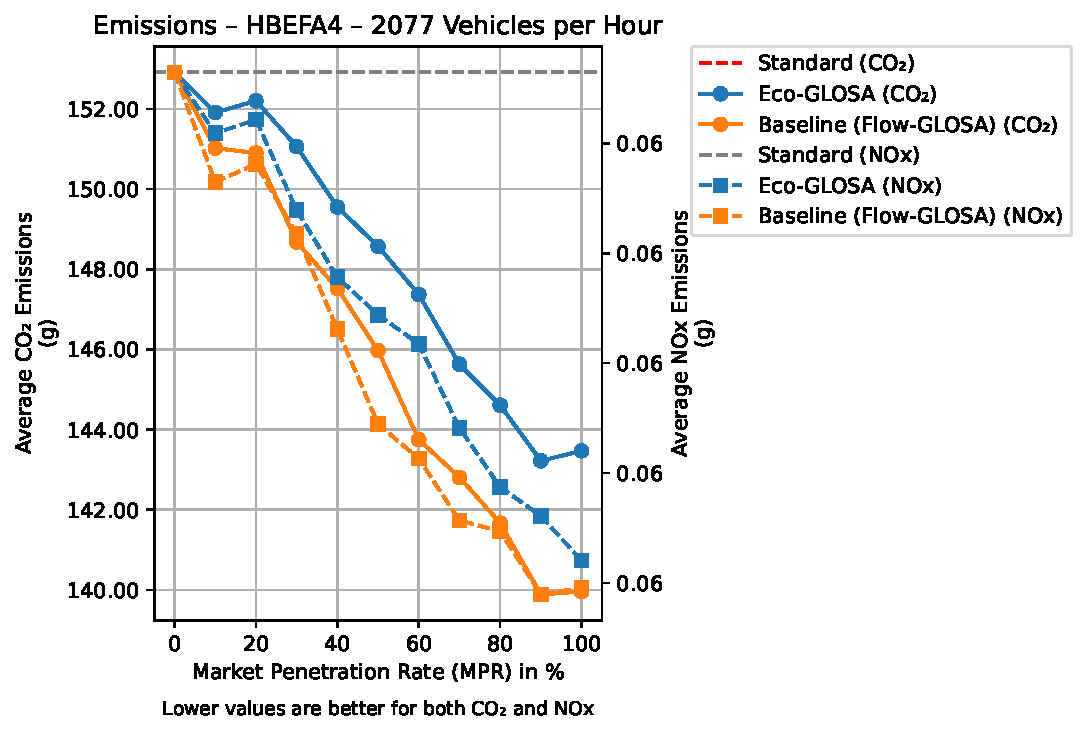
\includegraphics[width=\textwidth]{data/img/Emissions/Emissions_HBEFA4_Cars2077.pdf}
    \caption{HBEFA4 at $2077\,\mathrm{veh/h}$.}
    \label{fig:Emis_2077_HBEFA4}
  \end{subfigure}\hfill
  \begin{subfigure}[b]{0.45\textwidth}
    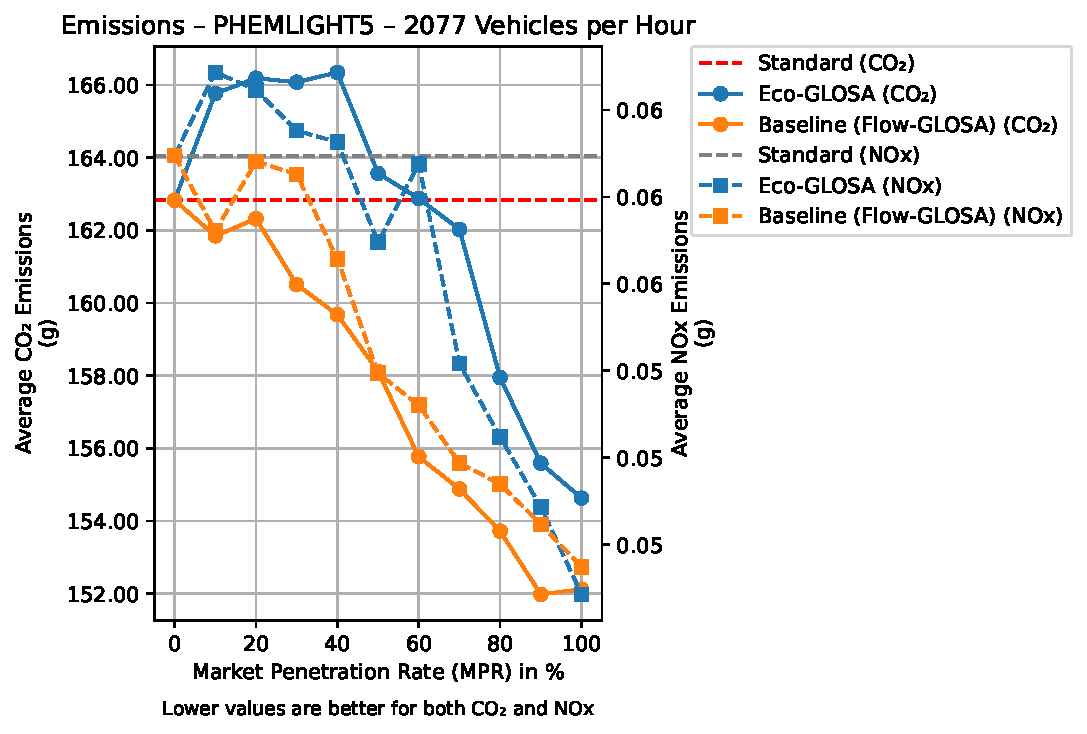
\includegraphics[width=\textwidth]{data/img/Emissions/Emissions_PHEMLIGHT5_Cars2077.pdf}
    \caption{PHEMlight5 at $2077\,\mathrm{veh/h}$.}
    \label{fig:Emis_2077_PHEM}
  \end{subfigure}
  \caption[\ac{co2} and \ac{nox} emissions vs. \ac{mpr} at $2077~\unit{\veh\per\hour}$]{\ac{co2} and \ac{nox} emissions versus \ac{mpr} under emerging congestion at $2077~\unit{\veh\per\hour}$.}
  \label{fig:Emis_2077}
\end{figure}

\paragraph{High Demand ($2769~\unit{\veh\per\hour}$).}
The demand level of $2769~\unit{\veh\per\hour}$ represents a critical turning point for the HBEFA4 model, where the \ac{eco-glosa} controller's performance collapses at moderate penetration rates. Instead of improvements, this leads to enormous emission spikes. The most severe outlier occurs at $60\%$ \ac{mpr}, where \ac{co2} emissions jump to $419.09~\unit{\gram\per\kilo\metre}$ and \ac{nox} emissions to $0.173~\unit{\gram\per\kilo\metre}$, representing increases of $164\%$ and $159\%$ over the Standard, respectively. A secondary peak in \ac{co2} emissions of $270.93~\unit{\gram\per\kilo\metre}$ is already present at $30\%$ \ac{mpr}. As seen in Figure~\vref{fig:Emis_2769_HBEFA4}, these excursions correspond to severe stop-and-go waves. In contrast, the \ac{flow-glosa} controller's emissions remain bounded and consistently below the Standard, showcasing its superior stability.
\mynewline
Under the PHEMlight5 model, the traffic jam is fully established at this demand, leading to poor performance for the \ac{eco-glosa} controller across all penetration rates. Its \ac{co2} emissions rise from the Standard of $168.29~\unit{\gram\per\kilo\metre}$ to a peak of $347.73~\unit{\gram\per\kilo\metre}$ at $70\%$ \ac{mpr}. Unlike the erratic spikes seen in the HBEFA4 model, PHEMlight5 predicts a more uniformly high emission profile for \ac{eco-glosa} in this congested state. This disparity stems from the PHEMlight5 model’s detailed transient engine maps, which impose a steep penalty on the inefficient, low-speed, high-load conditions that characterize a persistent traffic jam. As vehicles repeatedly accelerate from a standstill, their engines are forced into inefficient operating zones, inflating both fuel burn and \ac{nox} formation far beyond the forecasts of the HBEFA4 model.

\begin{figure}[htb]
  \centering
  \begin{subfigure}[b]{0.45\textwidth}
    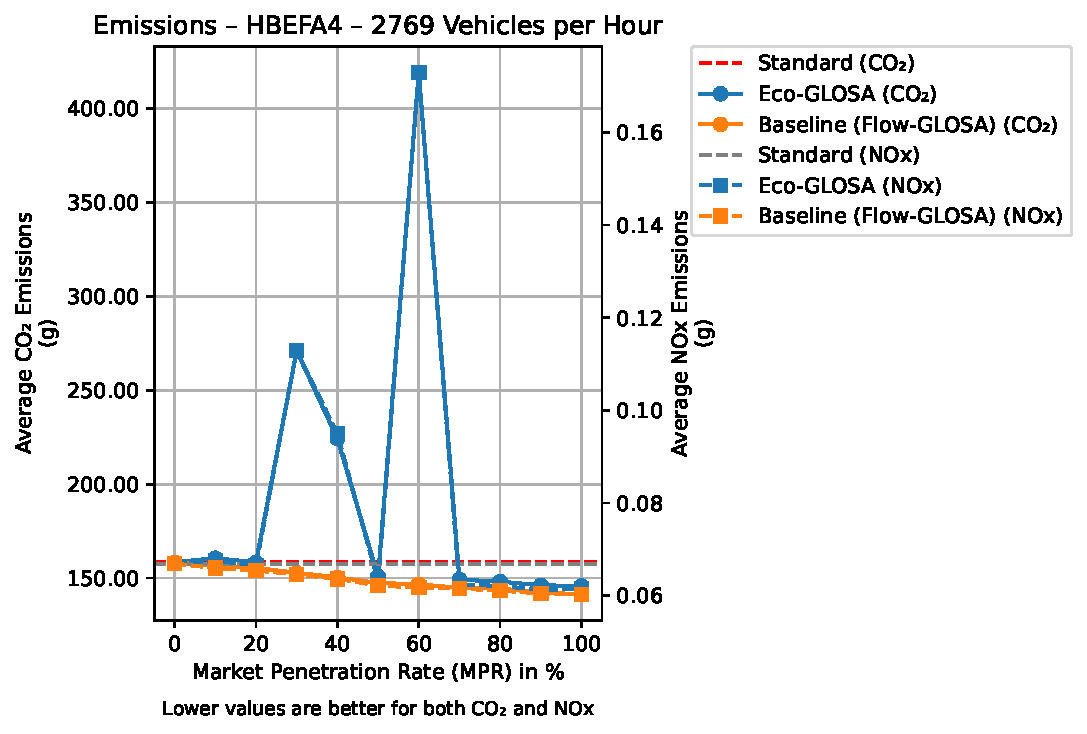
\includegraphics[width=\textwidth]{data/img/Emissions/Emissions_HBEFA4_Cars2769.pdf}
    \caption{HBEFA4 at $2769\,\mathrm{veh/h}$.}
    \label{fig:Emis_2769_HBEFA4}
  \end{subfigure}\hfill
  \begin{subfigure}[b]{0.45\textwidth}
    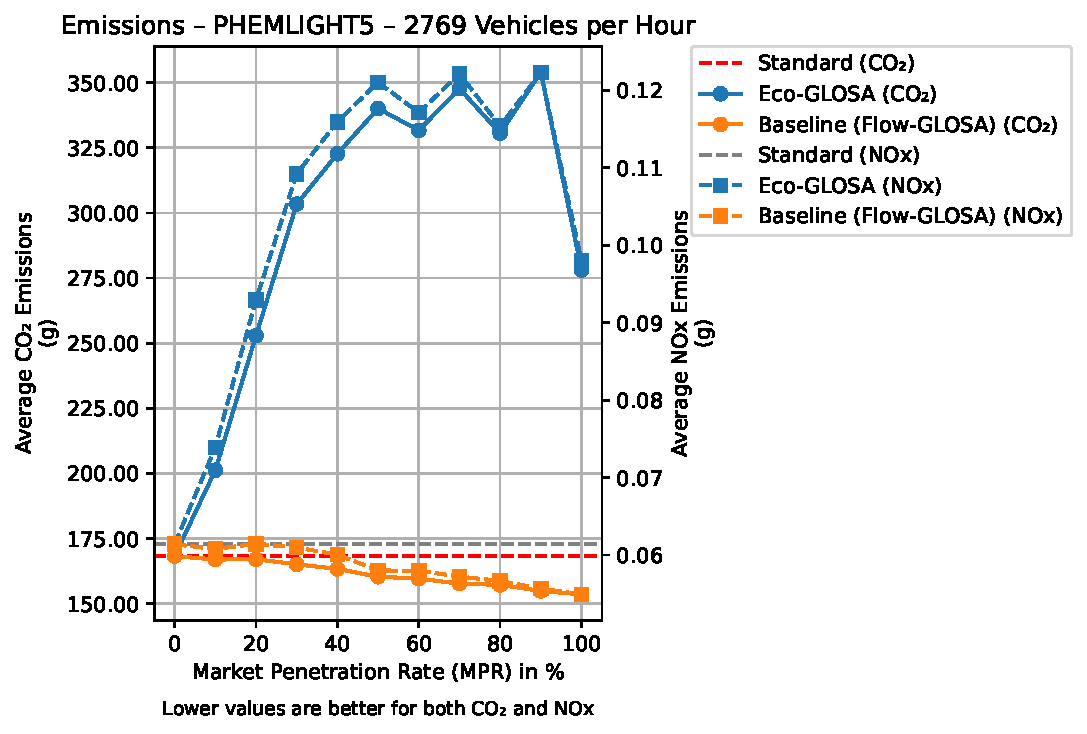
\includegraphics[width=\textwidth]{data/img/Emissions/Emissions_PHEMLIGHT5_Cars2769.pdf}
    \caption{PHEMlight5 at $2769\,\mathrm{veh/h}$.}
    \label{fig:Emis_2769_PHEM}
  \end{subfigure}
  \caption[\ac{co2} and \ac{nox} emissions vs. \ac{mpr} at $2769~\unit{\veh\per\hour}$]{\ac{co2} and \ac{nox} emissions versus \ac{mpr} at a high demand of $2769~\unit{\veh\per\hour}$, showing significant performance degradation for \ac{eco-glosa}.}
  \label{fig:Emis_2769}
\end{figure}

\paragraph{Saturated Regime ($3462~\unit{\veh\per\hour}$).}
The dichotomy between the two control philosophies is most striking in the fully saturated scenario, as shown in Figure~\vref{fig:Emis_3462}. Under the HBEFA4 model, the \ac{eco-glosa} controller consistently degrades performance as penetration increases. Its \ac{co2} emissions soar from the already high Standard of $426.68~\unit{\gram\per\kilo\metre}$ to a peak of $607.47~\unit{\gram\per\kilo\metre}$ at $80\%$ \ac{mpr}. Simultaneously, \ac{nox} emissions escalate dramatically from $0.175$ to $1.325~\unit{\gram\per\kilo\metre}$ at full penetration. This poor performance can be attributed to the controller's logic, which prioritises reaching the intersection for a green light, forcing futile and aggressive accelerations within an existing jam.
\mynewline
Conversely, the \ac{flow-glosa} controller drives the traffic jam to extinction. Under HBEFA4, its application causes \ac{co2} emissions to plummet from $426.68~\unit{\gram\per\kilo\metre}$ to just $151.33~\unit{\gram\per\kilo\metre}$ at $100\%$ \ac{mpr}. Once the queue clears, emissions settle on a plateau as vehicles traverse the corridor at a stable free-flow speed. This advantage is even more pronounced with the PHEMlight5 model. At full penetration, \ac{eco-glosa} still produces $367.78~\unit{\gram\per\kilo\metre}$ of \ac{co2}, whereas \ac{flow-glosa} emits only $152.59~\unit{\gram\per\kilo\metre}$. The absolute difference of $215.19~\unit{\gram\per\kilo\metre}$ represents a performance factor of $2.4$ in favour of the \ac{flow-glosa} strategy. A similar ratio is observed for \ac{nox} emissions ($0.829$ versus $0.341~\unit{\gram\per\kilo\metre}$). These findings reveal that a control law aimed at maximising throughput can dramatically outperform an ostensibly eco-oriented variant in heavily congested traffic.

\begin{figure}[htb]
  \centering
  \begin{subfigure}[b]{0.45\textwidth}
    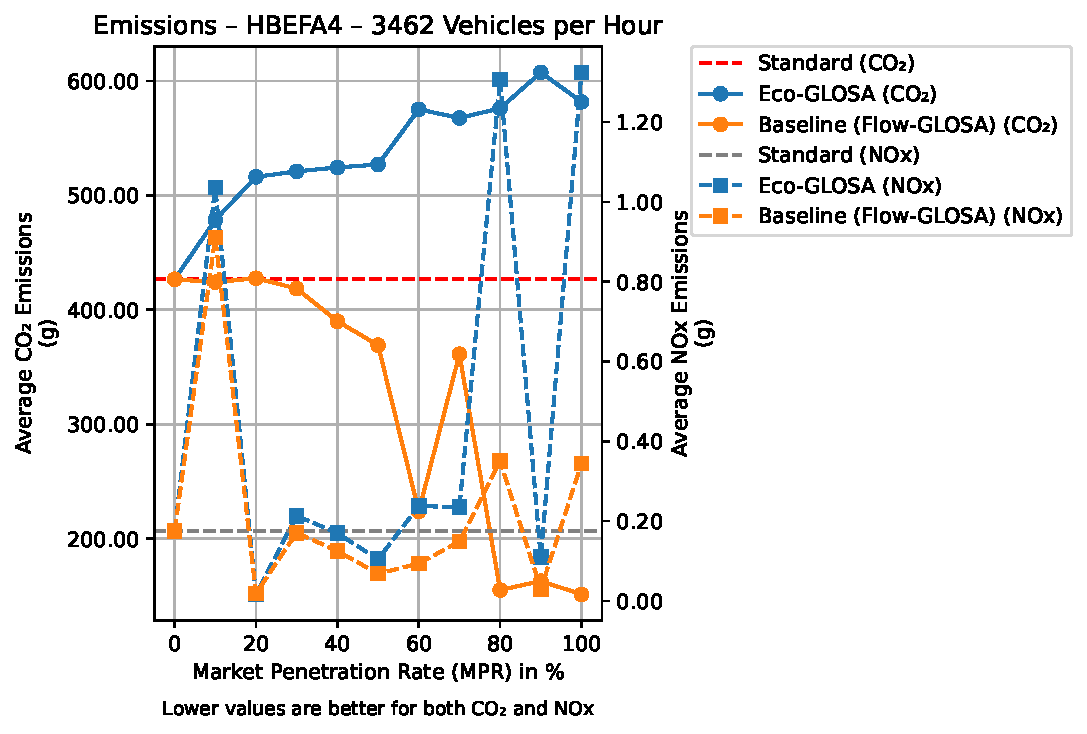
\includegraphics[width=\textwidth]{data/img/Emissions/Emissions_HBEFA4_Cars3462.pdf}
    \caption{HBEFA4 at $3462\,\mathrm{veh/h}$.}
    \label{fig:Emis_3462_HBEFA4}
  \end{subfigure}\hfill
  \begin{subfigure}[b]{0.45\textwidth}
    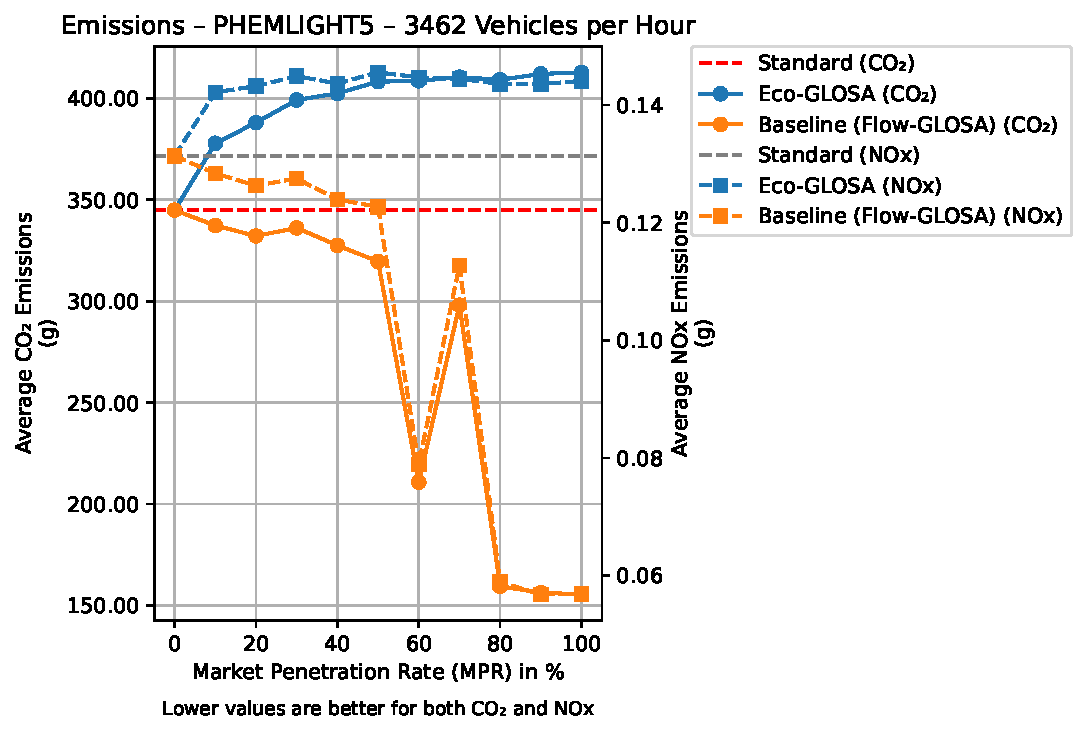
\includegraphics[width=\textwidth]{data/img/Emissions/Emissions_PHEMLIGHT5_Cars3462.pdf}
    \caption{PHEMlight5 at $3462\,\mathrm{veh/h}$.}
    \label{fig:Emis_3462_PHEM}
  \end{subfigure}
  \caption[\ac{co2} and \ac{nox} emissions vs. \ac{mpr} at $3462~\unit{\veh\per\hour}$]{\ac{co2} and \ac{nox} emissions versus \ac{mpr} in the fully saturated regime ($3462~\unit{\veh\per\hour}$), highlighting the superior performance of \ac{flow-glosa}.}
  \label{fig:Emis_3462}
\end{figure}

\paragraph{Inter-Model Comparison.}
Juxtaposing the HBEFA4 and PHEMlight5 models reveals two key differences in their predictions. First, they provide different estimates of the absolute benefits of \ac{flow-glosa} in saturation. For the $3462~\unit{\veh\per\hour}$ scenario, HBEFA4 predicts a \ac{co2} reduction of approximately $64\%$, while PHEMlight5 estimates a more conservative, though still substantial, $56\%$ reduction. This discrepancy arises because the Standard (baseline) emission value for HBEFA4 is inflated by more than $80~\unit{\gram\per\kilo\metre}$ compared to PHEMlight5, suggesting its static drive-cycle factors may inadequately capture engine behaviour during prolonged idling.
\mynewline
Second, the models diverge in their sensitivity to the performance degradation of \ac{eco-glosa} in congested traffic. At $2769~\unit{\veh\per\hour}$, the PHEMlight5 model shows that \ac{eco-glosa} becomes detrimental almost immediately, yielding higher emissions than \ac{flow-glosa} from just $10\%$ \ac{mpr} onwards. The HBEFA4 results are more volatile, showing severe emission spikes at certain penetration rates rather than a consistent trend. The earlier and more consistent penalty from PHEMlight5 is likely explained by its more granular power-band binning, which better captures the inefficiency of the aggressive, transient manoeuvres induced by \ac{eco-glosa} in dense traffic.

\paragraph{Key Conclusions on Emissions.}
The emission analysis reveals that a single \ac{glosa} strategy is not universally optimal; performance is highly dependent on traffic density. In under-saturated traffic, the emission impact is often dominated by stochastic effects, with neither controller showing a consistent advantage. As congestion becomes moderate, both algorithms can reduce \ac{co2} and \ac{nox} emissions, with \ac{eco-glosa} offering the greatest potential improvements provided that traffic oscillations remain mild.
\mynewline
Beyond a critical volume threshold, however, the myopic nature of the \ac{eco-glosa} controller becomes a significant liability. Its focus on individual vehicle efficiency amplifies stop-and-go waves, in some cases more than doubling emissions. This effect is so pronounced that, particularly when evaluated with the sensitive PHEMlight5 model, the introduction of \ac{eco-glosa} can \textit{induce a severe traffic jam} in conditions that would otherwise remain free-flowing. In these high-density scenarios, a throughput-centered strategy like \ac{flow-glosa} proves superior. By resolving the jam entirely at an \ac{mpr} of $80\%$ or higher, it can cut emissions by over $60\%$ compared to the Standard case. Ultimately, the choice of emission model is critical, as the higher fidelity of PHEMlight5 predicts these performance shifts more accurately than the HBEFA4 model.
\mynewline
This underscores a key methodological paradox concerning the choice of emission model. The high physical fidelity of PHEMlight5 accurately penalises the severe energy cost of transient, stop-and-go manoeuvres. In response, the \ac{eco-glosa} controller, in its strict pursuit of minimising fuel use, advises overly conservative speed profiles to avoid these high-cost states. Paradoxically, this locally optimal strategy is what induces severe network-level congestion, creating traffic jams where none existed and ultimately leading to far higher system-wide emissions. In contrast, the HBEFA4 model's relative insensitivity to these transient states leads to speed advisories that, while less \enquote{eco-optimal} in a narrow sense, are more compatible with maintaining traffic flow. The result is that the less accurate model, when paired with the \ac{eco-glosa} controller, leads to a better overall environmental outcome precisely because it prevents the controller from making decisions that are disastrous for network stability. This finding suggests that a successful eco-driving controller must balance high-fidelity physical models with robust, network-level traffic flow objectives to prevent locally optimal choices from causing globally detrimental effects.

\begin{table}[htb]
  \centering
  \caption[Average \ac{co2} and \ac{nox} emissions for all traffic volumes and \acp{mpr}]{Vehicle emissions in terms of average \ac{co2} ($\unit{\gram\per\kilo\metre}$) and \ac{nox} ($\unit{\gram\per\kilo\metre}$) for all traffic volumes and \acp{mpr}. The data compares the Standard, \ac{flow-glosa}, and \ac{eco-glosa} configurations.}
  \label{tab:Emissions}
  \resizebox{\textwidth}{!}{%
    \begin{tabular}{l l l *{11}{c}}
      \toprule
      Vehicles & Algorithm                & Fuel         & \textbf{0 \% (Standard)} & 10 \%     & 20 \%     & 30 \%       & 40 \%       & 50 \%       & 60 \%       & 70 \%       & 80 \%       & 90 \%       & 100 \%      \\
      \midrule
      69.0 & Eco-GLOSA                 & HBEFA4       & \textbf{149.99,0.0606}   & 164.05,0.03 & 169.37,0.0345 & 144.59,0.0582 & \textbf{127.88,0.0167} & 165.55,0.0342 & 143.45,0.0549 & 141.49,0.0555 & 154.28,0.0286 & 147.82,0.355  & 153.20,0.3521 \\
      69.0 & Baseline (Flow-GLOSA)     & HBEFA4       & \textbf{149.99,0.0606}   & 164.58,0.0302 & 171.67,0.0349 & 145.27,0.0588 & 128.53,0.0171 & 162.00,0.0332 & 145.08,0.0563 & 140.88,0.0548 & 153.86,0.0287 & 145.60,0.3528 & 149.80,0.3543 \\
      69.0 & Eco-GLOSA                 & PHEMlight5   & \textbf{155.51,0.0586}   & 156.20,0.0331 & \textbf{148.83,0.0358} & 148.37,0.0515 & 142.98,0.0199 & \textbf{131.45,0.0312} & 149.17,0.0552 & 144.54,0.0493 & 138.25,0.0296 & 136.50,0.3026 & 137.57,0.3034 \\
      69.0 & Baseline (Flow-GLOSA)     & PHEMlight5   & \textbf{155.51,0.0586}   & 150.06,0.0328 & 148.80,0.0367 & 150.51,0.0534 & 145.63,0.0215 & 138.77,0.0330 & 150.43,0.0531 & 147.89,0.0504 & 139.57,0.0291 & 141.36,0.3147 & 154.08,0.3891 \\
      \midrule
      138.0 & Eco-GLOSA                & HBEFA4       & \textbf{148.70,0.0653}   & 158.42,0.3739 & 142.81,0.0521 & 144.14,0.0660 & 142.15,0.0172 & 131.18,0.0215 & 141.96,0.0650 & 140.59,0.0634 & 161.97,0.3757 & 163.17,0.0337 & 146.68,0.3450 \\
      138.0 & Baseline (Flow-GLOSA)    & HBEFA4       & \textbf{148.70,0.0653}   & 151.97,0.3579 & 143.07,0.0522 & 145.54,0.0669 & 137.95,0.0169 & 133.02,0.0216 & 141.83,0.0661 & 139.88,0.0638 & 157.35,0.3669 & 168.69,0.0342 & 147.16,0.3522 \\
      138.0 & Eco-GLOSA                & PHEMlight5   & \textbf{155.28,0.0603}   & 155.68,0.3546 & 162.40,0.0403 & 149.91,0.0623 & 151.66,0.0208 & 144.26,0.0185 & 148.81,0.0583 & 147.75,0.0577 & 150.13,0.3467 & 136.40,0.0323 & 142.41,0.3166 \\
      138.0 & Baseline (Flow-GLOSA)    & PHEMlight5   & \textbf{155.28,0.0603}   & 150.74,0.3583 & 160.31,0.0409 & 153.54,0.0635 & 153.58,0.0224 & 148.65,0.0185 & 150.68,0.0638 & 148.26,0.0610 & 156.77,0.3734 & 144.61,0.0352 & 145.27,0.3295 \\
      \midrule
      346.0 & Eco-GLOSA                & HBEFA4       & \textbf{147.86,0.0613}   & 166.00,0.0303 & 135.38,0.0165 & 147.48,0.0607 & 153.16,0.3518 & 131.61,0.0150 & 142.92,0.0591 & 144.14,0.0596 & 159.45,0.0293 & 168.06,0.0348 & 162.48,0.0337 \\
      346.0 & Baseline (Flow-GLOSA)    & HBEFA4       & \textbf{147.86,0.0613}   & 164.34,0.0301 & 137.57,0.0163 & 146.00,0.0605 & 151.92,0.3526 & 132.37,0.0158 & 142.70,0.0592 & 142.98,0.0597 & 156.50,0.0288 & 166.58,0.0348 & 162.83,0.0342 \\
      346.0 & Eco-GLOSA                & PHEMlight5   & \textbf{156.60,0.0565}   & 143.04,0.0307 & 147.53,0.0193 & 155.81,0.0555 & 153.46,0.3496 & 147.79,0.0177 & 151.95,0.0540 & 151.23,0.0533 & 143.46,0.0302 & 141.59,0.0341 & 143.35,0.0348 \\
      346.0 & Baseline (Flow-GLOSA)    & PHEMlight5   & \textbf{156.60,0.0565}   & 151.50,0.0326 & 152.03,0.0201 & 155.66,0.0570 & 150.87,0.3398 & 147.92,0.0181 & 152.34,0.0549 & 152.69,0.0553 & 145.78,0.0311 & 147.78,0.0358 & 145.27,0.0356 \\
      \midrule
      692.0 & Eco-GLOSA                & HBEFA4       & \textbf{148.06,0.0611}   & 168.31,0.0314 & 146.24,0.0533 & 145.79,0.0608 & 139.15,0.0397 & 143.76,0.0524 & 142.99,0.0596 & 143.02,0.0588 & 166.96,0.0306 & 144.01,0.0141 & 161.09,0.0298 \\
      692.0 & Baseline (Flow-GLOSA)    & HBEFA4       & \textbf{148.06,0.0611}   & 179.99,0.0336 & 147.31,0.0537 & 145.89,0.0608 & 138.17,0.0393 & 144.78,0.0529 & 142.14,0.0592 & 141.76,0.0585 & 161.27,0.0299 & 141.95,0.0146 & 155.71,0.0287 \\
      692.0 & Eco-GLOSA                & PHEMlight5   & \textbf{157.36,0.0551}   & 156.92,0.0354 & 167.32,0.0424 & 157.20,0.0561 & 154.02,0.0298 & 163.01,0.0409 & 153.51,0.0546 & 152.85,0.0528 & 143.86,0.0318 & 143.84,0.0177 & 138.86,0.0299 \\
      692.0 & Baseline (Flow-GLOSA)    & PHEMlight5   & \textbf{157.36,0.0551}   & 164.91,0.0357 & 165.46,0.0422 & 156.18,0.0559 & 153.11,0.0297 & 162.90,0.0412 & 152.91,0.0544 & 152.79,0.0536 & 150.63,0.0331 & 145.53,0.0189 & 143.37,0.0310 \\
      \midrule
      1385.0 & Eco-GLOSA               & HBEFA4       & \textbf{149.86,0.0584}   & 137.88,0.0167 & 141.17,0.0403 & 147.99,0.0573 & 150.72,0.0157 & 153.69,0.3545 & 145.46,0.0562 & 144.34,0.0558 & 131.05,0.0145 & 167.72,0.0344 & \textbf{130.39,0.0141} \\
      1385.0 & Baseline (Flow-GLOSA)   & HBEFA4       & \textbf{149.86,0.0584}   & 138.62,0.0165 & 140.78,0.0402 & 147.28,0.0575 & 148.88,0.0156 & 153.32,0.3530 & 143.28,0.0561 & 142.33,0.0555 & 130.39,0.0155 & 168.69,0.0349 & 128.27,0.0154 \\
      1385.0 & Eco-GLOSA               & PHEMlight5   & \textbf{159.38,0.0528}   & 156.69,0.0206 & 158.86,0.0307 & 162.99,0.0548 & 156.69,0.0217 & 158.01,0.3604 & 160.70,0.0533 & 157.58,0.0508 & 154.07,0.0182 & 150.49,0.0365 & \textbf{148.21,0.0164} \\
      1385.0 & Baseline (Flow-GLOSA)   & PHEMlight5   & \textbf{159.38,0.0528}   & 155.23,0.0210 & 155.04,0.0300 & 158.16,0.0532 & 151.80,0.0209 & 153.21,0.3538 & 154.51,0.0519 & 153.93,0.0509 & 148.74,0.0187 & 149.63,0.0360 & 146.85,0.0180 \\
      \midrule
      2077.0 & Eco-GLOSA               & HBEFA4       & \textbf{152.91,0.0616}   & 141.32,0.0163 & 171.95,0.0317 & 151.06,0.0604 & 158.07,0.3611 & 157.57,0.3599 & 147.37,0.0592 & 145.63,0.0584 & 132.87,0.0138 & 145.67,0.0138 & \textbf{133.30,0.0138} \\
      2077.0 & Baseline (Flow-GLOSA)   & HBEFA4       & \textbf{152.91,0.0616}   & 141.43,0.0161 & 168.98,0.0314 & 148.68,0.0602 & 157.28,0.3600 & 153.32,0.3523 & 143.75,0.0581 & 142.81,0.0576 & 131.22,0.0153 & 143.94,0.0145 & 129.17,0.0152 \\
      2077.0 & Eco-GLOSA               & PHEMlight5   & \textbf{162.83,0.0565}   & 162.24,0.0215 & 165.20,0.0369 & 166.08,0.0568 & 161.99,0.3670 & 159.59,0.3623 & 162.88,0.0564 & 162.03,0.0541 & 157.46,0.0180 & 152.18,0.0185 & \textbf{154.31,0.0163} \\
      2077.0 & Baseline (Flow-GLOSA)   & PHEMlight5   & \textbf{162.83,0.0565}   & 158.18,0.0207 & 157.42,0.0348 & 160.51,0.0563 & 158.86,0.3637 & 154.02,0.3506 & 155.77,0.0536 & 154.88,0.0529 & 150.66,0.0189 & 148.04,0.0195 & 148.71,0.0182 \\
      \midrule
      2769.0 & Eco-GLOSA               & HBEFA4       & \textbf{158.44,0.0669}   & 149.68,0.0165 & 150.27,0.0438 & \textbf{270.93,0.1129} & 223.93,0.0152 & 144.07,0.0419 & \textbf{419.09,0.1730} & 149.20,0.0624 & 136.94,0.0136 & 137.47,0.0233 & \textbf{134.94,0.0131} \\
      2769.0 & Baseline (Flow-GLOSA)   & HBEFA4       & \textbf{158.44,0.0669}   & 144.45,0.0163 & 148.28,0.0431 & 152.84,0.0646 & 155.17,0.0153 & 140.40,0.0405 & 146.67,0.0617 & 144.90,0.0615 & 133.43,0.0148 & 134.78,0.0224 & 131.03,0.0145 \\
      2769.0 & Eco-GLOSA               & PHEMlight5   & \textbf{168.29,0.0614}   & 191.39,0.0278 & 232.01,0.0462 & 303.40,0.1092 & 284.24,0.0441 & 306.10,0.0621 & 331.67,0.1171 & \textbf{347.73,0.1221} & 295.95,0.0404 & 321.37,0.0433 & \textbf{255.90,0.0318} \\
      2769.0 & Baseline (Flow-GLOSA)   & PHEMlight5   & \textbf{168.29,0.0614}   & 161.20,0.0215 & 162.91,0.0316 & 165.15,0.0610 & 158.91,0.0223 & 157.16,0.0305 & 159.67,0.0580 & 157.75,0.0572 & 153.28,0.0188 & 153.69,0.0194 & 150.97,0.0179 \\
      \midrule
      3462.0 & Eco-GLOSA               & HBEFA4       & \textbf{426.68,0.1747}   & 478.55,1.0357 & 516.15,0.0163 & 520.98,0.2133 & 524.40,0.1698 & 526.96,0.1042 & 575.15,0.2378 & 567.63,0.2347 & \textbf{607.47,0.1096} & 581.74,0.1096 & \textbf{581.74,1.3247} \\
      3462.0 & Baseline (Flow-GLOSA)   & HBEFA4       & \textbf{426.68,0.1747}   & 424.17,0.9106 & 427.59,0.0187 & 418.54,0.1707 & 389.99,0.1248 & 369.14,0.0681 & \textbf{223.84,0.0933} & 361.16,0.1486 & \textbf{155.09,0.3505} & \textbf{162.90,0.0296} & \textbf{151.33,0.3443} \\
      3462.0 & Eco-GLOSA               & PHEMlight5   & \textbf{344.88,0.1313}   & 361.38,0.8343 & 343.20,0.0563 & 399.19,0.1449 & 357.12,0.0729 & 369.50,0.0461 & 408.63,0.1447 & 410.45,0.1445 & \textbf{364.90,0.8214} & 359.41,0.0796 & \textbf{367.78,0.8285} \\
      3462.0 & Baseline (Flow-GLOSA)   & PHEMlight5   & \textbf{344.88,0.1313}   & 329.05,0.7561 & 299.05,0.0511 & 336.12,0.1275 & 297.39,0.0604 & 297.18,0.0321 & 210.82,0.0789 & 298.02,0.1127 & \textbf{156.83,0.3529} & \textbf{151.75,0.0330} & \textbf{152.59,0.3409} \\
      \bottomrule
    \end{tabular}%
  }
\end{table}
